\section{Multiphase Fluid Dynamics and Root Zone Aeration in Lunar Gravity}
\label{sec:fluid_dynamics}

\subsection{Fractional Gravity and Capillary Dominance}
\label{subsec:fractional_gravity}

Fluid dynamics in terrestrial soils reflect an equilibrium between gravitational drainage and capillary matric suction\cite{steinberg2007fluid,jones1999microgravity}. On the lunar surface, gravitational acceleration drops to $g_L \approx 1.62\,\mathrm{m/s}^2$, precisely one-sixth of terrestrial gravity ($g_E \approx 9.81\,\mathrm{m/s}^2$)\cite{ming1989lunar}. This reduction fundamentally alters the dimensionless Bond number ($\mathrm{Bo}$), which defines the ratio of gravitational body forces to interfacial capillary surface tension forces within a porous medium\cite{ming1989lunar,ostrach1982low}:
\begin{equation}
    \mathrm{Bo} = \frac{\Delta\rho \cdot g \cdot d^2}{\gamma}
    \label{eq:bond_number}
\end{equation}
where $\Delta\rho$ is the density difference between the liquid nutrient solution and the habitat atmosphere ($\mathrm{kg/m}^3$), $g$ is the local gravitational acceleration ($\mathrm{m/s}^2$), $d$ is the characteristic pore-throat diameter ($\mathrm{m}$), and $\gamma$ is the liquid-gas surface tension ($\mathrm{N/m}$)\cite{ming1989lunar,jones1999microgravity}.

Because lunar gravity is reduced by a factor of 6 while the surface tension of aqueous nutrient solutions remains effectively constant, the Bond number decreases by nearly an order of magnitude\cite{ming1989lunar,ostrach1982low,podolskiy2005capillary}. Consequently, the hydraulic regime transitions from gravity-assisted drainage to capillary-dominated retention\cite{ming1989lunar,podolskiy2005capillary}. The theoretical equilibrium height of capillary rise ($h_c$) is described by the Young-Laplace equation:
\begin{equation}
    h_c = \frac{2\gamma \cos\theta}{\rho g r}
    \label{eq:capillary_rise}
\end{equation}
where $\theta$ is the fluid contact angle, $\rho$ is fluid density, and $r$ is the effective pore radius\cite{ming1989lunar,steinberg2007fluid,jones1999microgravity}.

Because $g$ is situated in the denominator, the height of the capillary fringe increases six-fold for any given pore size compared to Earth\cite{ming1989lunar}. In unsorted, polydisperse raw lunar regolith, this shift creates severe hydraulic dysfunctions\cite{paul2022plants,ming1989lunar,podolskiy2005capillary}. Natural regolith exhibits a broad particle size distribution spanning from sub-micrometer dust to millimeter-sized rock fragments, yielding an uncontrolled, heterogeneous pore network\cite{paul2022plants,turci2015mechanistic}. Under $1/6\,g$, capillary forces trap water in the abundant fine micropores ($<10\,\mu\mathrm{m}$), establishing an expansive saturated zone that acts as a physical barrier to gas exchange\cite{paul2022plants,ming1989lunar}. Simultaneously, larger pores ($>100\,\mu\mathrm{m}$) drain erratically or form bypass dry channels\cite{ming1989lunar,podolskiy2005capillary}. As a consequence, the root zone experiences rapid hypoxia, suffocating aerobic root respiration, arresting mitochondrial ATP production via oxidative phosphorylation, and fostering root rot\cite{ming1989lunar,podolskiy2005capillary,massa2024controlled}.

\subsection{Pore Architecture Engineering and Matric Potential Control}
\label{subsec:pore_engineering}

Engineered thermal sintering overcomes these hydraulic barriers by providing direct control over substrate pore architecture\cite{ming1989lunar,heinse2007porous,jones2002liquid}. Prior to thermal consolidation, raw regolith is sieved to isolate a classified particle size fraction, specifically grains between $45$ and $75\,\mu\mathrm{m}$\cite{ming1989lunar}. Sintering this uniform fraction produces porous ceramic bodies with interconnected pore throat diameters concentrated between $30$ and $60\,\mu\mathrm{m}$, and total open porosities of $35\text{--}42\%$\cite{ming1989lunar}.

This engineered pore-size distribution optimizes the substrate's soil-water retention curve, governed by the van Genuchten constitutive formulation\cite{jones2002liquid,heinse2007measurement}:
\begin{equation}
    \Theta(h) = \frac{\theta(h) - \theta_r}{\theta_s - \theta_r} = \left[ 1 + \left(\alpha |h|\right)^n \right]^{-m}
    \label{eq:van_genuchten}
\end{equation}
where $\Theta(h)$ is the normalized volumetric water content, $\theta(h)$ is volumetric moisture content, $\theta_r$ and $\theta_s$ are residual and saturated water contents, $h$ is matric suction head ($\mathrm{cm}$ or $\mathrm{kPa}$), and $\alpha, n$, and $m = 1 - 1/n$ are empirical shape parameters determined by pore network geometry\cite{jones2002liquid,heinse2007measurement}.

By eliminating both ultra-fine micropores ($<5\,\mu\mathrm{m}$) that induce waterlogging and macropores ($>150\,\mu\mathrm{m}$) that trigger premature drainage, sintered ceramics stabilize matric suction within an optimal operating window of $-2.5$ to $-5.0\,\mathrm{kPa}$ (Figure~\ref{fig:hydrodynamics_aeration} and Table~\ref{tab:hydraulic_properties})\cite{ming1989lunar}. This suction is sufficient to wick nutrient solutions across the root zone against fractional gravity, yet low enough to allow plant roots to absorb water with minimal metabolic energy expenditure\cite{ming1989lunar}. Crucially, this pore architecture maintains air-filled porosity above $25\text{--}30\%$ at field capacity under $1/6\,g$\cite{ming1989lunar,heinse2007porous,podolskiy2005capillary}. This open gas network supports continuous diffusive oxygen transport to root cell boundaries, matching root respiration and canopy transpiration rates observed in terrestrial hydroponic systems\cite{ming1989lunar,wheeler2023space,podolskiy2005capillary}.

\begin{figure}[t!]
    \centering
    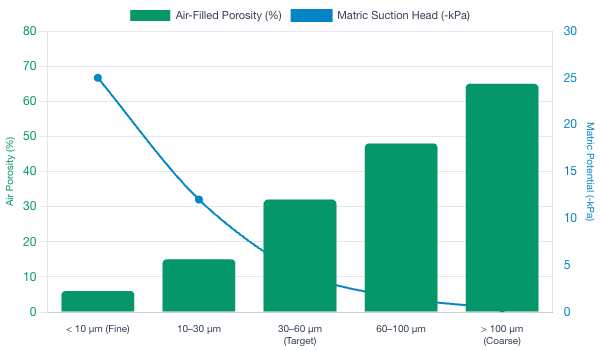
\includegraphics[width=0.88\textwidth]{figures/fig3_hydrodynamics_aeration.png}
    \caption{\textbf{Multiphase fluid dynamics and root zone aeration in fractional lunar gravity ($1/6\,g$).} Relationship between pore throat diameter ($\mu\mathrm{m}$), air-filled porosity (\%, green bars), and matric suction head ($-\mathrm{kPa}$, blue line). Below $30\,\mu\mathrm{m}$, capillary trapping induces waterlogging and severe hypoxia risk ($<15\%$ air porosity). Above $60\,\mu\mathrm{m}$, weak capillary suction leads to dry channeling. The engineered $30\text{--}60\,\mu\mathrm{m}$ pore window balances capillary liquid wicking with $>25\text{--}30\%$ air-filled porosity for aerobic root respiration.}
    \label{fig:hydrodynamics_aeration}
\end{figure}

\begin{table}[t!]
\small
\centering
\caption{\textbf{Comparison of hydraulic, physical, and transport parameters in raw lunar regolith versus sintered engineered ceramics under $1/6\,g$.}}
\label{tab:hydraulic_properties}
\begin{tabularx}{\textwidth}{lXXX}
\toprule
\textbf{Hydraulic / Physical Parameter} & \textbf{Raw Lunar Regolith Bed} & \textbf{Sintered Engineered Ceramic} & \textbf{Physiological \& Systemic Impact} \\
\midrule
Grain Size Distribution & Polydisperse ($<1\,\mu\mathrm{m}$ to $1000\,\mu\mathrm{m}$)\cite{ming1989lunar,lytvynenko2021lunar} & Classified, sorted fraction ($45\text{--}75\,\mu\mathrm{m}$)\cite{ming1989lunar} & Eliminates packing collapse and dry channeling\cite{ming1989lunar} \\
\addlinespace
Pore Throat Diameter ($d_\mathrm{pore}$) & Uncontrolled ($0.1\,\mu\mathrm{m}$ to $250\,\mu\mathrm{m}$)\cite{paul2022plants,ming1989lunar} & Monodisperse control ($30\text{--}60\,\mu\mathrm{m}$)\cite{ming1989lunar} & Stabilizes capillary wicking without fluid entrapment\cite{ming1989lunar} \\
\addlinespace
Matric Potential Window ($\psi_m$) & Unstable ($-0.1$ to $<-100\,\mathrm{kPa}$)\cite{ming1989lunar,hendrix2024reactivity} & Controlled ($-2.5$ to $-5.0\,\mathrm{kPa}$)\cite{ming1989lunar} & Matches root water uptake with minimal plant energy expenditure\cite{ming1989lunar,jones2002liquid} \\
\addlinespace
Air-Filled Porosity at Saturation & $<8\text{--}12\%$ (Severe hypoxia risk)\cite{paul2022plants,ming1989lunar} & $>25\text{--}30\%$ (Continuous aeration)\cite{ming1989lunar} & Maintains aerobic root respiration; prevents root decay\cite{ming1989lunar} \\
\addlinespace
Hydraulic Conductivity ($K_\mathrm{sat}$) & Spatially erratic; causes stagnant zones\cite{paul2022plants,podolskiy2005capillary} & Isotropic; stable convective mass transfer\cite{ming1989lunar} & Prevents localized fertilizer salt accumulation\cite{ming1989lunar,wamelink2024struvite} \\
\bottomrule
\end{tabularx}
\end{table}
